\section{Contagio sociale}
Le scelte di un agente possono riflettere, oltre al proprio, anche lo stato d'animo degli altri soggetti che popolano l'ambiente di interesse. Ogni atteggiamento che scaturisce da una persona può essere, in positivo quanto in negativo, causa della medesima risposta anche in un'altra. \newline
Alla base di questo principio, c'è il già citato meccanismo del contagio sociale, che ha nella trasmissione della paura il suo più lampante esempio. Vedendo un intero gruppo scappare terrorizzato, infatti, la reazione spontanea per un essere umano è quella di fare altrettanto, anche se non si è riscontrata presenza concreta del pericolo.

\subsection{Descrizione della simulazione}
In un ambiente euclideo continuo ed illimitato, vengono definite una zona di sicurezza ed una di pericolo da parti opposte e sono caricati, nello spazio compreso tra esse, due raggruppamenti di pedoni rispettivamente costituiti da 75 e 25 persone. \newline 
Mentre il gruppo più numeroso, costituito da pedoni cognitivi, viene posizionato in prossimità del pericolo, quello meno numeroso è collocato a debita distanza da esso. Nonostante la distanza, la traiettoria da seguire per raggiungere il più velocemente possibile la zona di sicurezza è la stessa per entrambi. \newline
La simulazione è stata eseguita in due casi, differenziando la tipologia di pedone utilizzata per il gruppo da 25: eterogeneo nella prima, cognitivo nella seconda.

\subsection{Risultati ottenuti}
Come è possibile osservare dai momenti significativi raccolti in figura \ref{fig:social-contagion-not-cognitive}, i pedoni eterogenei, trovandosi lontani e non potendo percepire direttamente il pericolo, rimangono al loro posto per tutto il decorrere della simulazione e osservano indifferenti il gruppo costituito dai 75 agenti cognitivi passargli vicino nell'intento di raggiungere la zona di sicurezza. \newline
Diversamente, valutando la situazione negli stessi istanti temporali, ma in presenza di soli agenti cognitivi (figura \ref{fig:social-contagion-cognitive}), possiamo notare come progressivamente anche il secondo gruppo, impaurito dallo stato emotivo dei pedoni del primo, inizi a scappare nella stessa direzione. 

\begin{figure}
    \centering
    \begin{subfigure}[b]{0.75\textwidth}
        \centering
        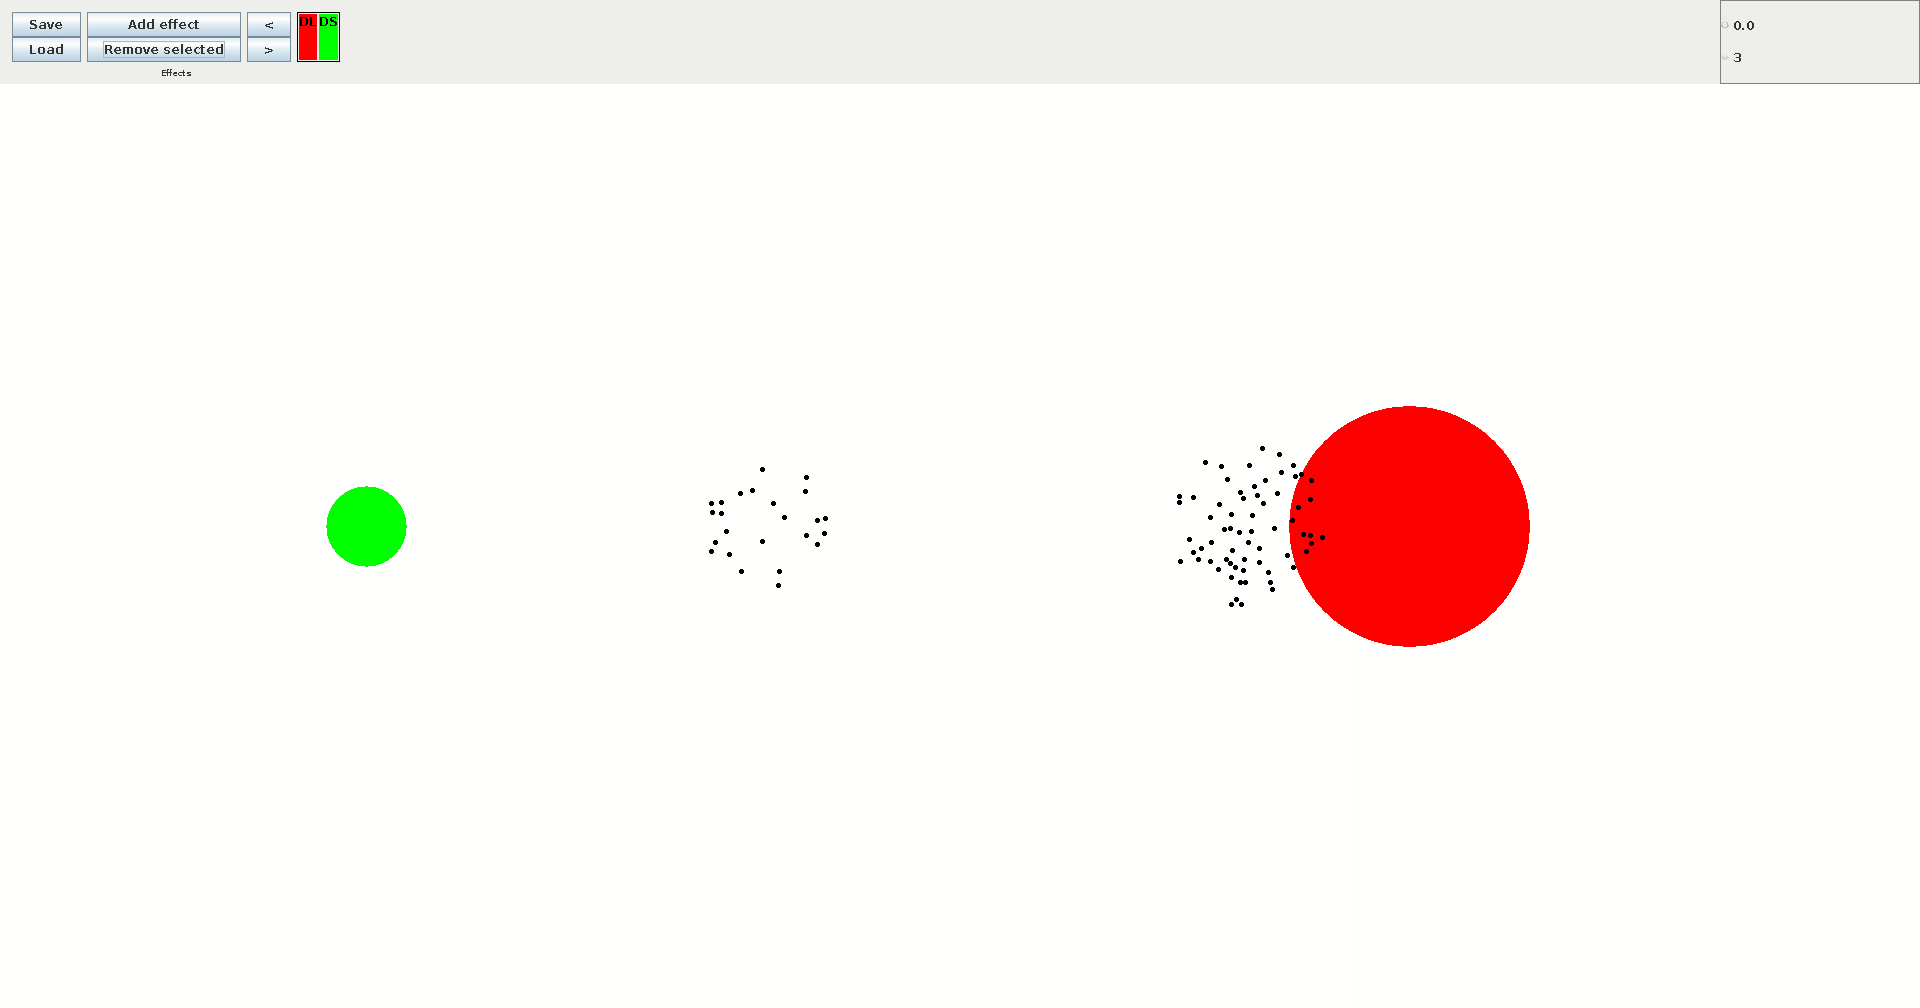
\includegraphics[width=\textwidth]{immagini/casi-studio/social-contagion-not-cognitive-begin.png}
    \end{subfigure}
    \hfill
    \begin{subfigure}[b]{0.75\textwidth}
        \centering
        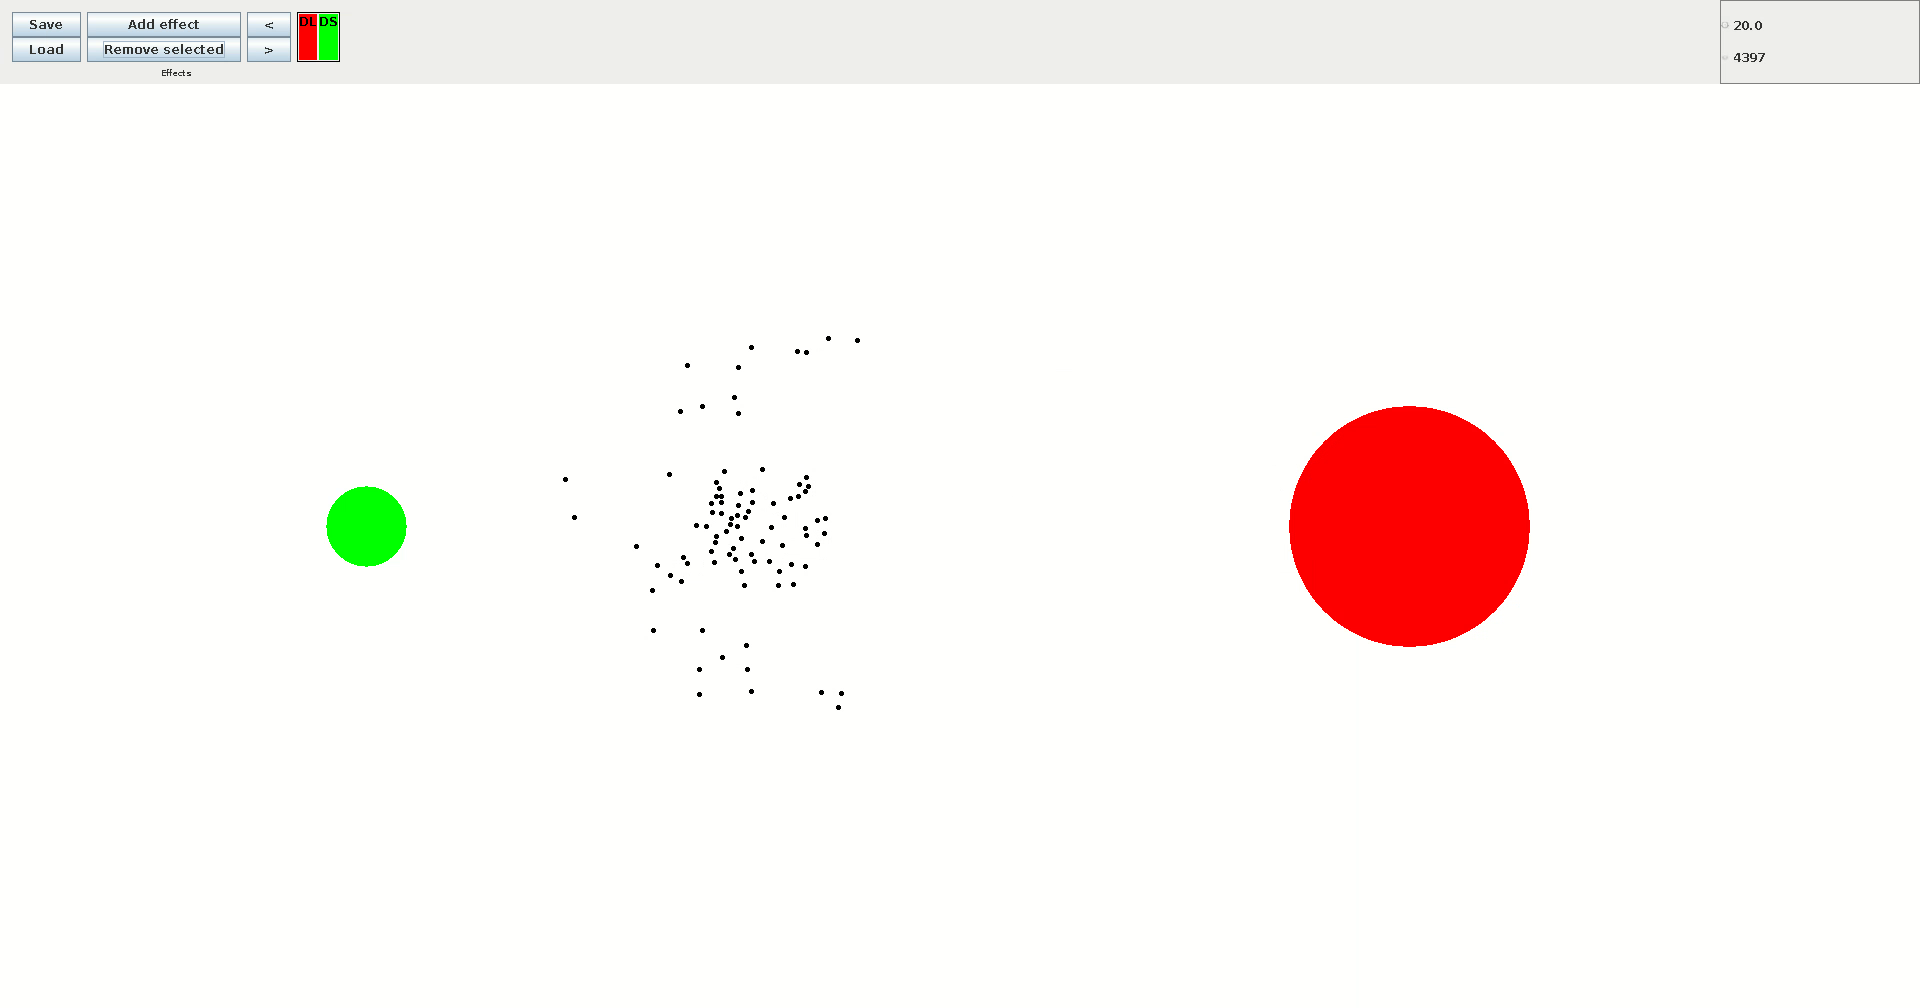
\includegraphics[width=\textwidth]{immagini/casi-studio/social-contagion-not-cognitive-during.png}
    \end{subfigure}
    \hfill
    \begin{subfigure}[b]{0.75\textwidth}
        \centering
        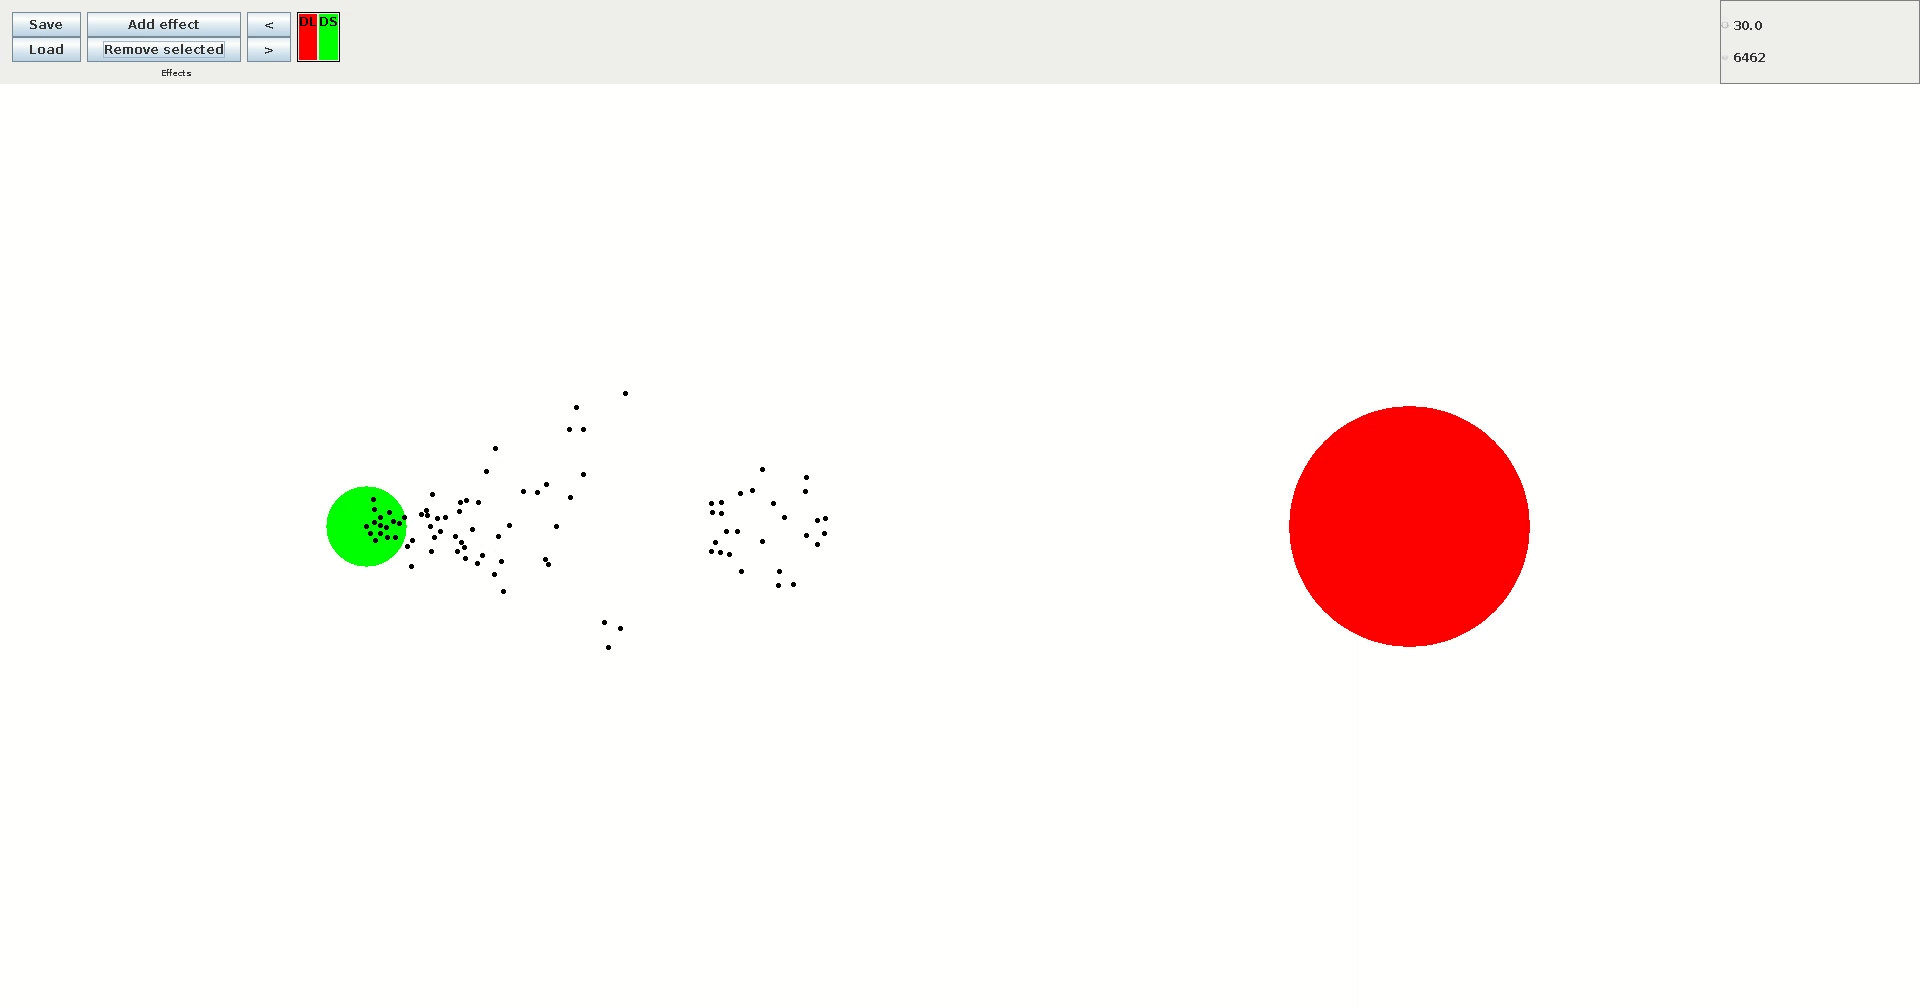
\includegraphics[width=\textwidth]{immagini/casi-studio/social-contagion-not-cognitive-end.png}
    \end{subfigure}
    \caption{Fotogrammi salienti della simulazione sul contagio sociale in presenza di pedoni non cognitivi; non avendo delle caratteristiche emotive e non potendo quindi percepire il panico degli agenti nel gruppo di destra, essi rimangono al loro posto.}
    \label{fig:social-contagion-not-cognitive}
\end{figure}

\begin{figure}
    \centering
    \begin{subfigure}[b]{0.75\textwidth}
        \centering
        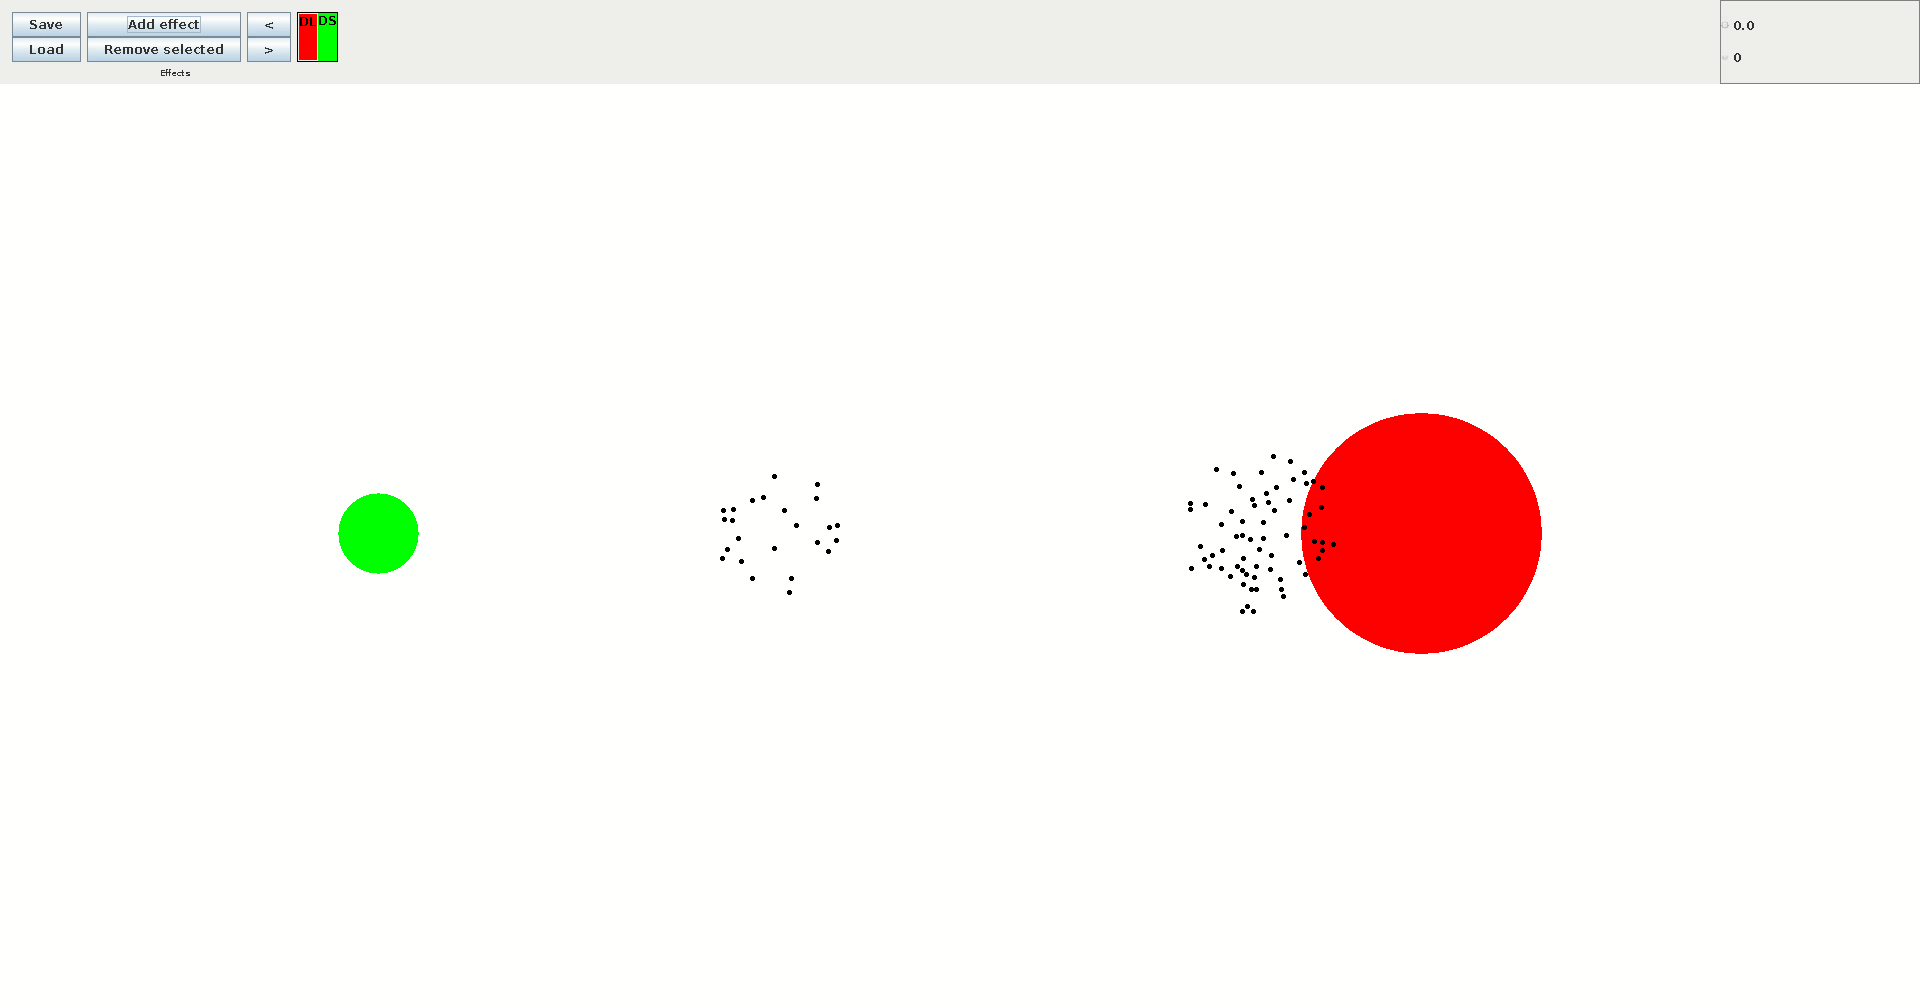
\includegraphics[width=\textwidth]{immagini/casi-studio/social-contagion-cognitive-begin.png}
    \end{subfigure}
    \hfill
    \begin{subfigure}[b]{0.75\textwidth}
        \centering
        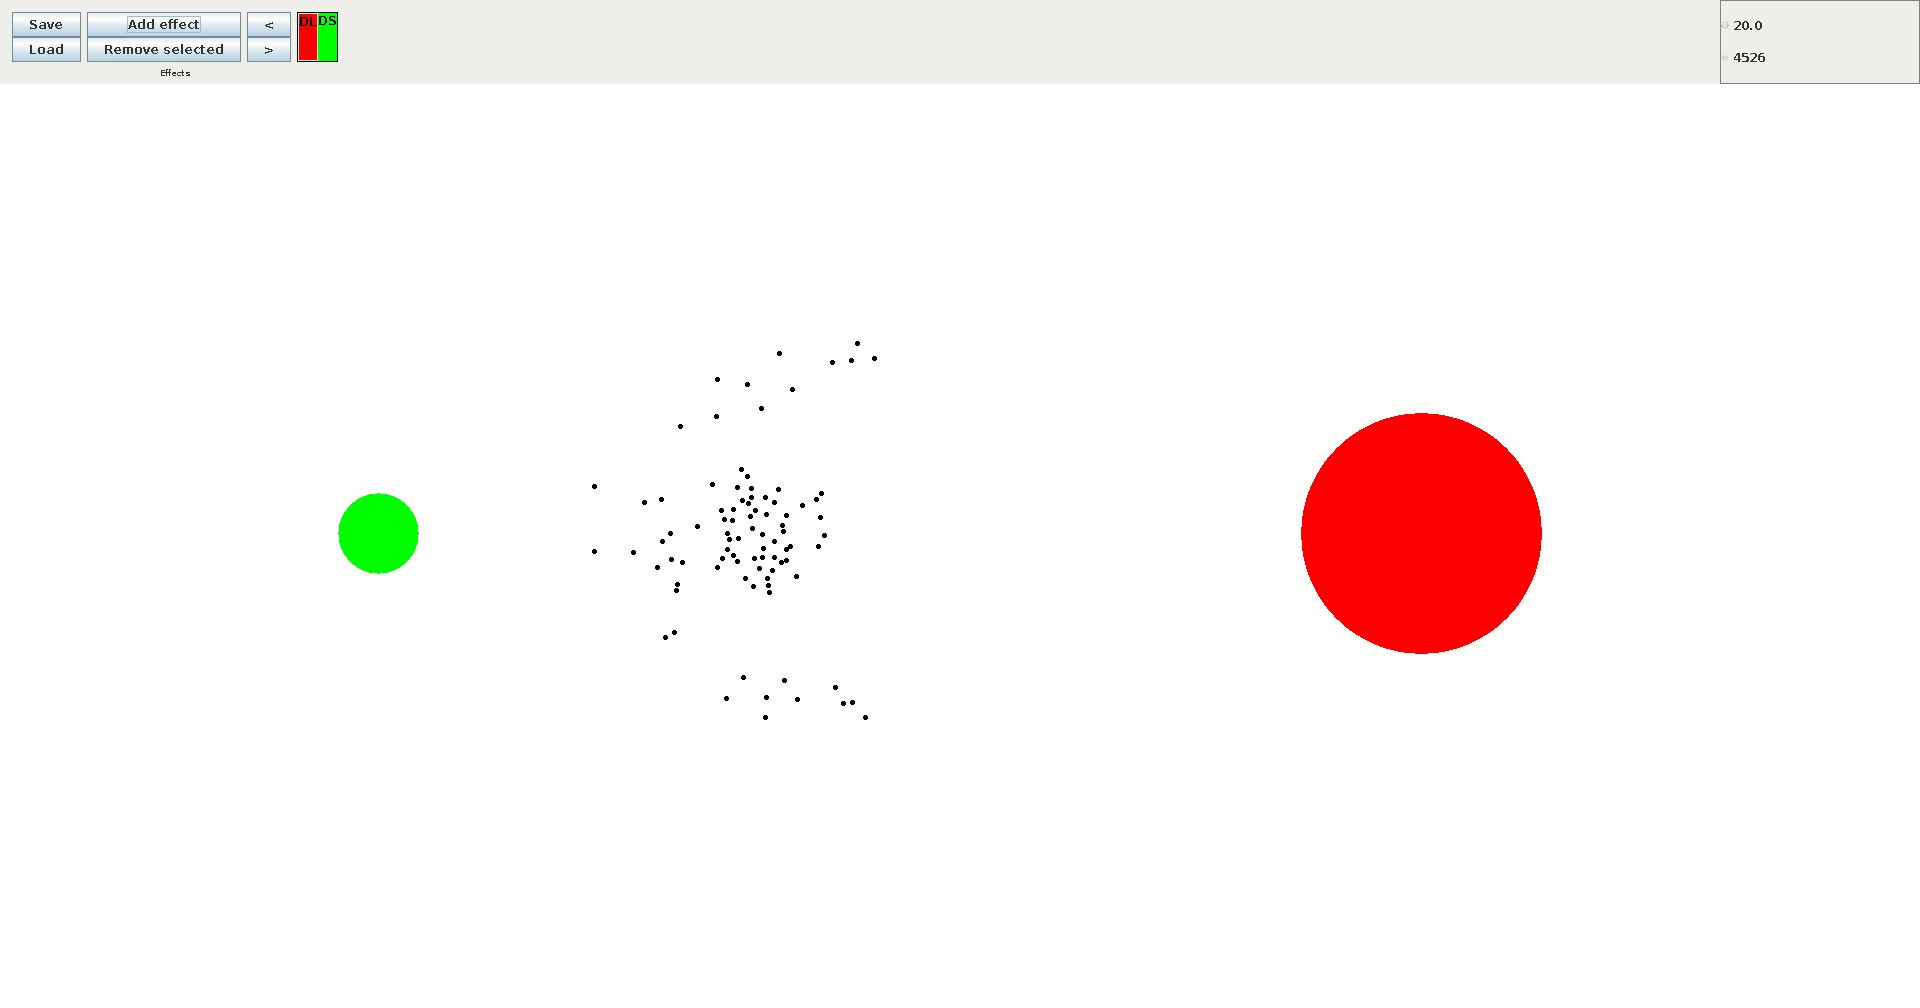
\includegraphics[width=\textwidth]{immagini/casi-studio/social-contagion-cognitive-during.png}
    \end{subfigure}
    \hfill
    \begin{subfigure}[b]{0.75\textwidth}
        \centering
        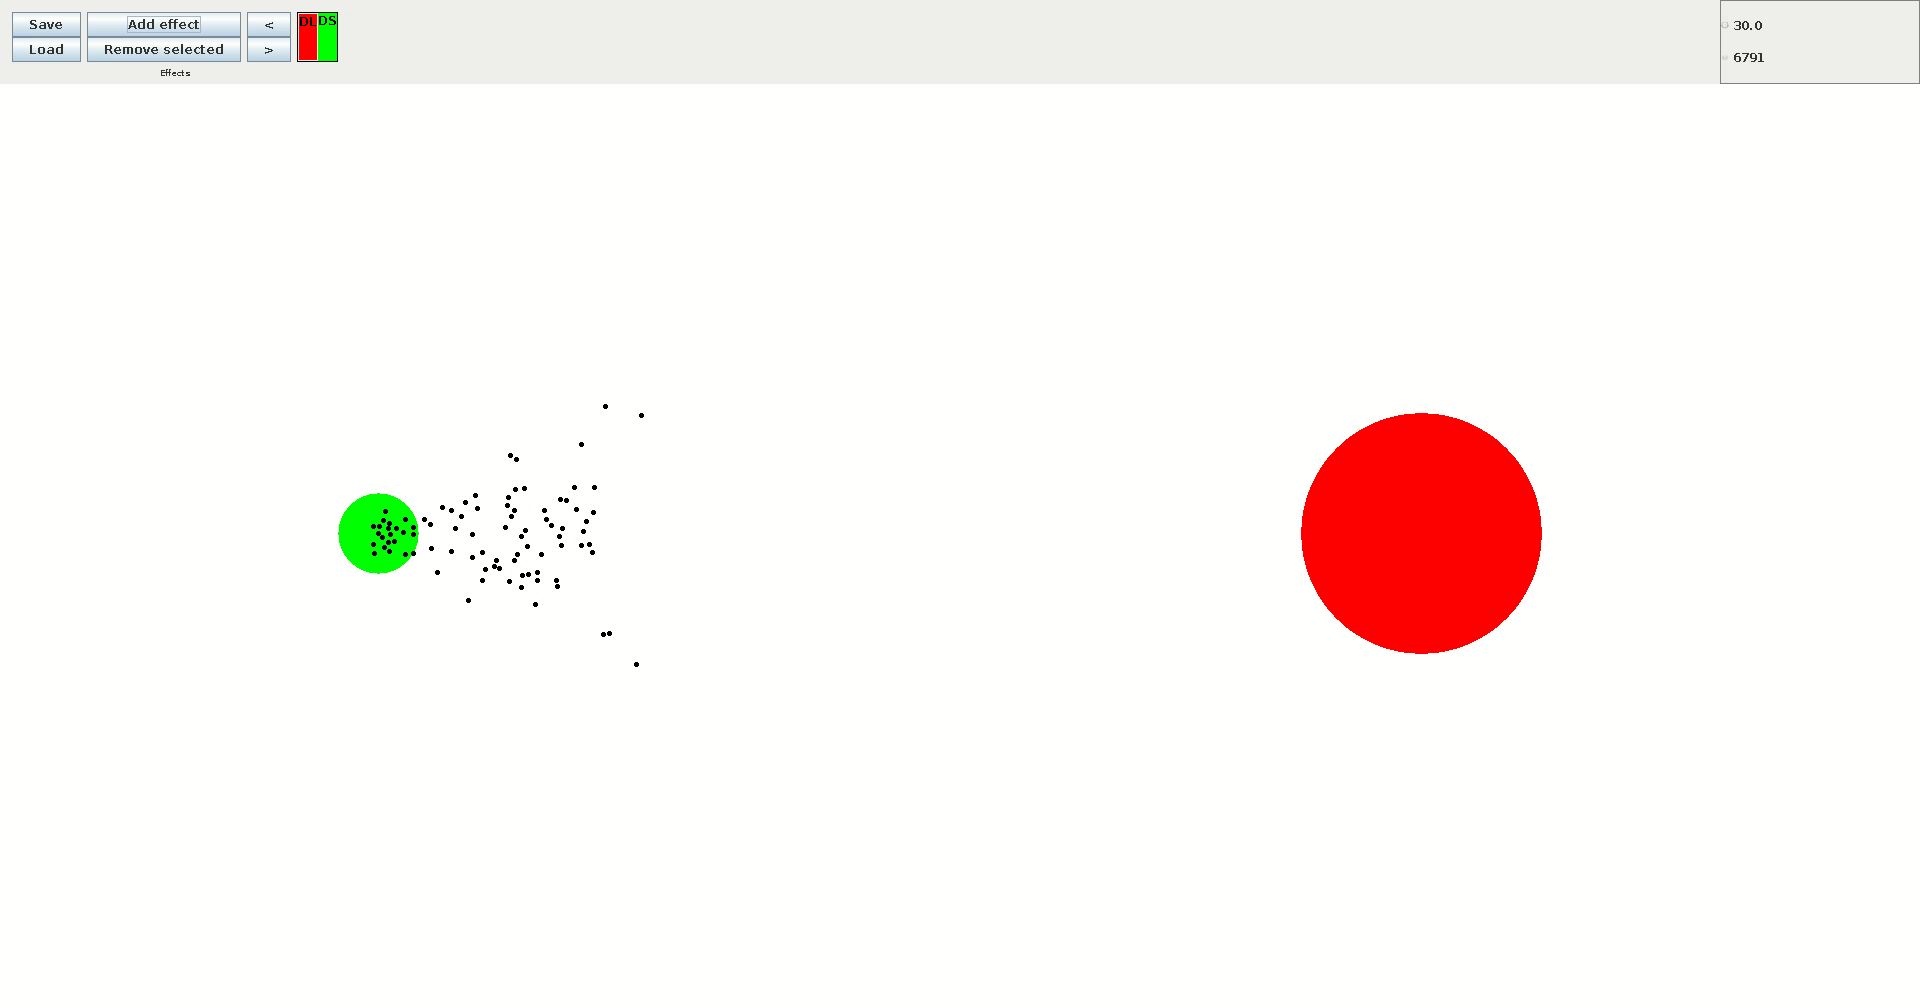
\includegraphics[width=\textwidth]{immagini/casi-studio/social-contagion-cognitive-end.png}
    \end{subfigure}
    \caption{Fotogrammi salienti della simulazione sul contagio sociale in presenza di pedoni cognitivi; il fenomeno della trasmissione del panico nel momento in cui i due gruppi si incrociano, porta gli agenti precedentemente fermi ad iniziare a fuggire.}
    \label{fig:social-contagion-cognitive}
\end{figure}